\section{div-biguint}
\label{div-biguint}

\begin{enumerate}
    \item target
        \begin{itemize}
            \item implenment the division of two biguints
        \end{itemize}
    \item constraints-logic
        \begin{itemize}
            \item compute mul-factors first, use U32ArithmeticGate
            \item add mul-factors from low bits, use U32AddManyGate
        \end{itemize}
    \item mul-process layout
        \begin{figure}[!ht]
            \centering
            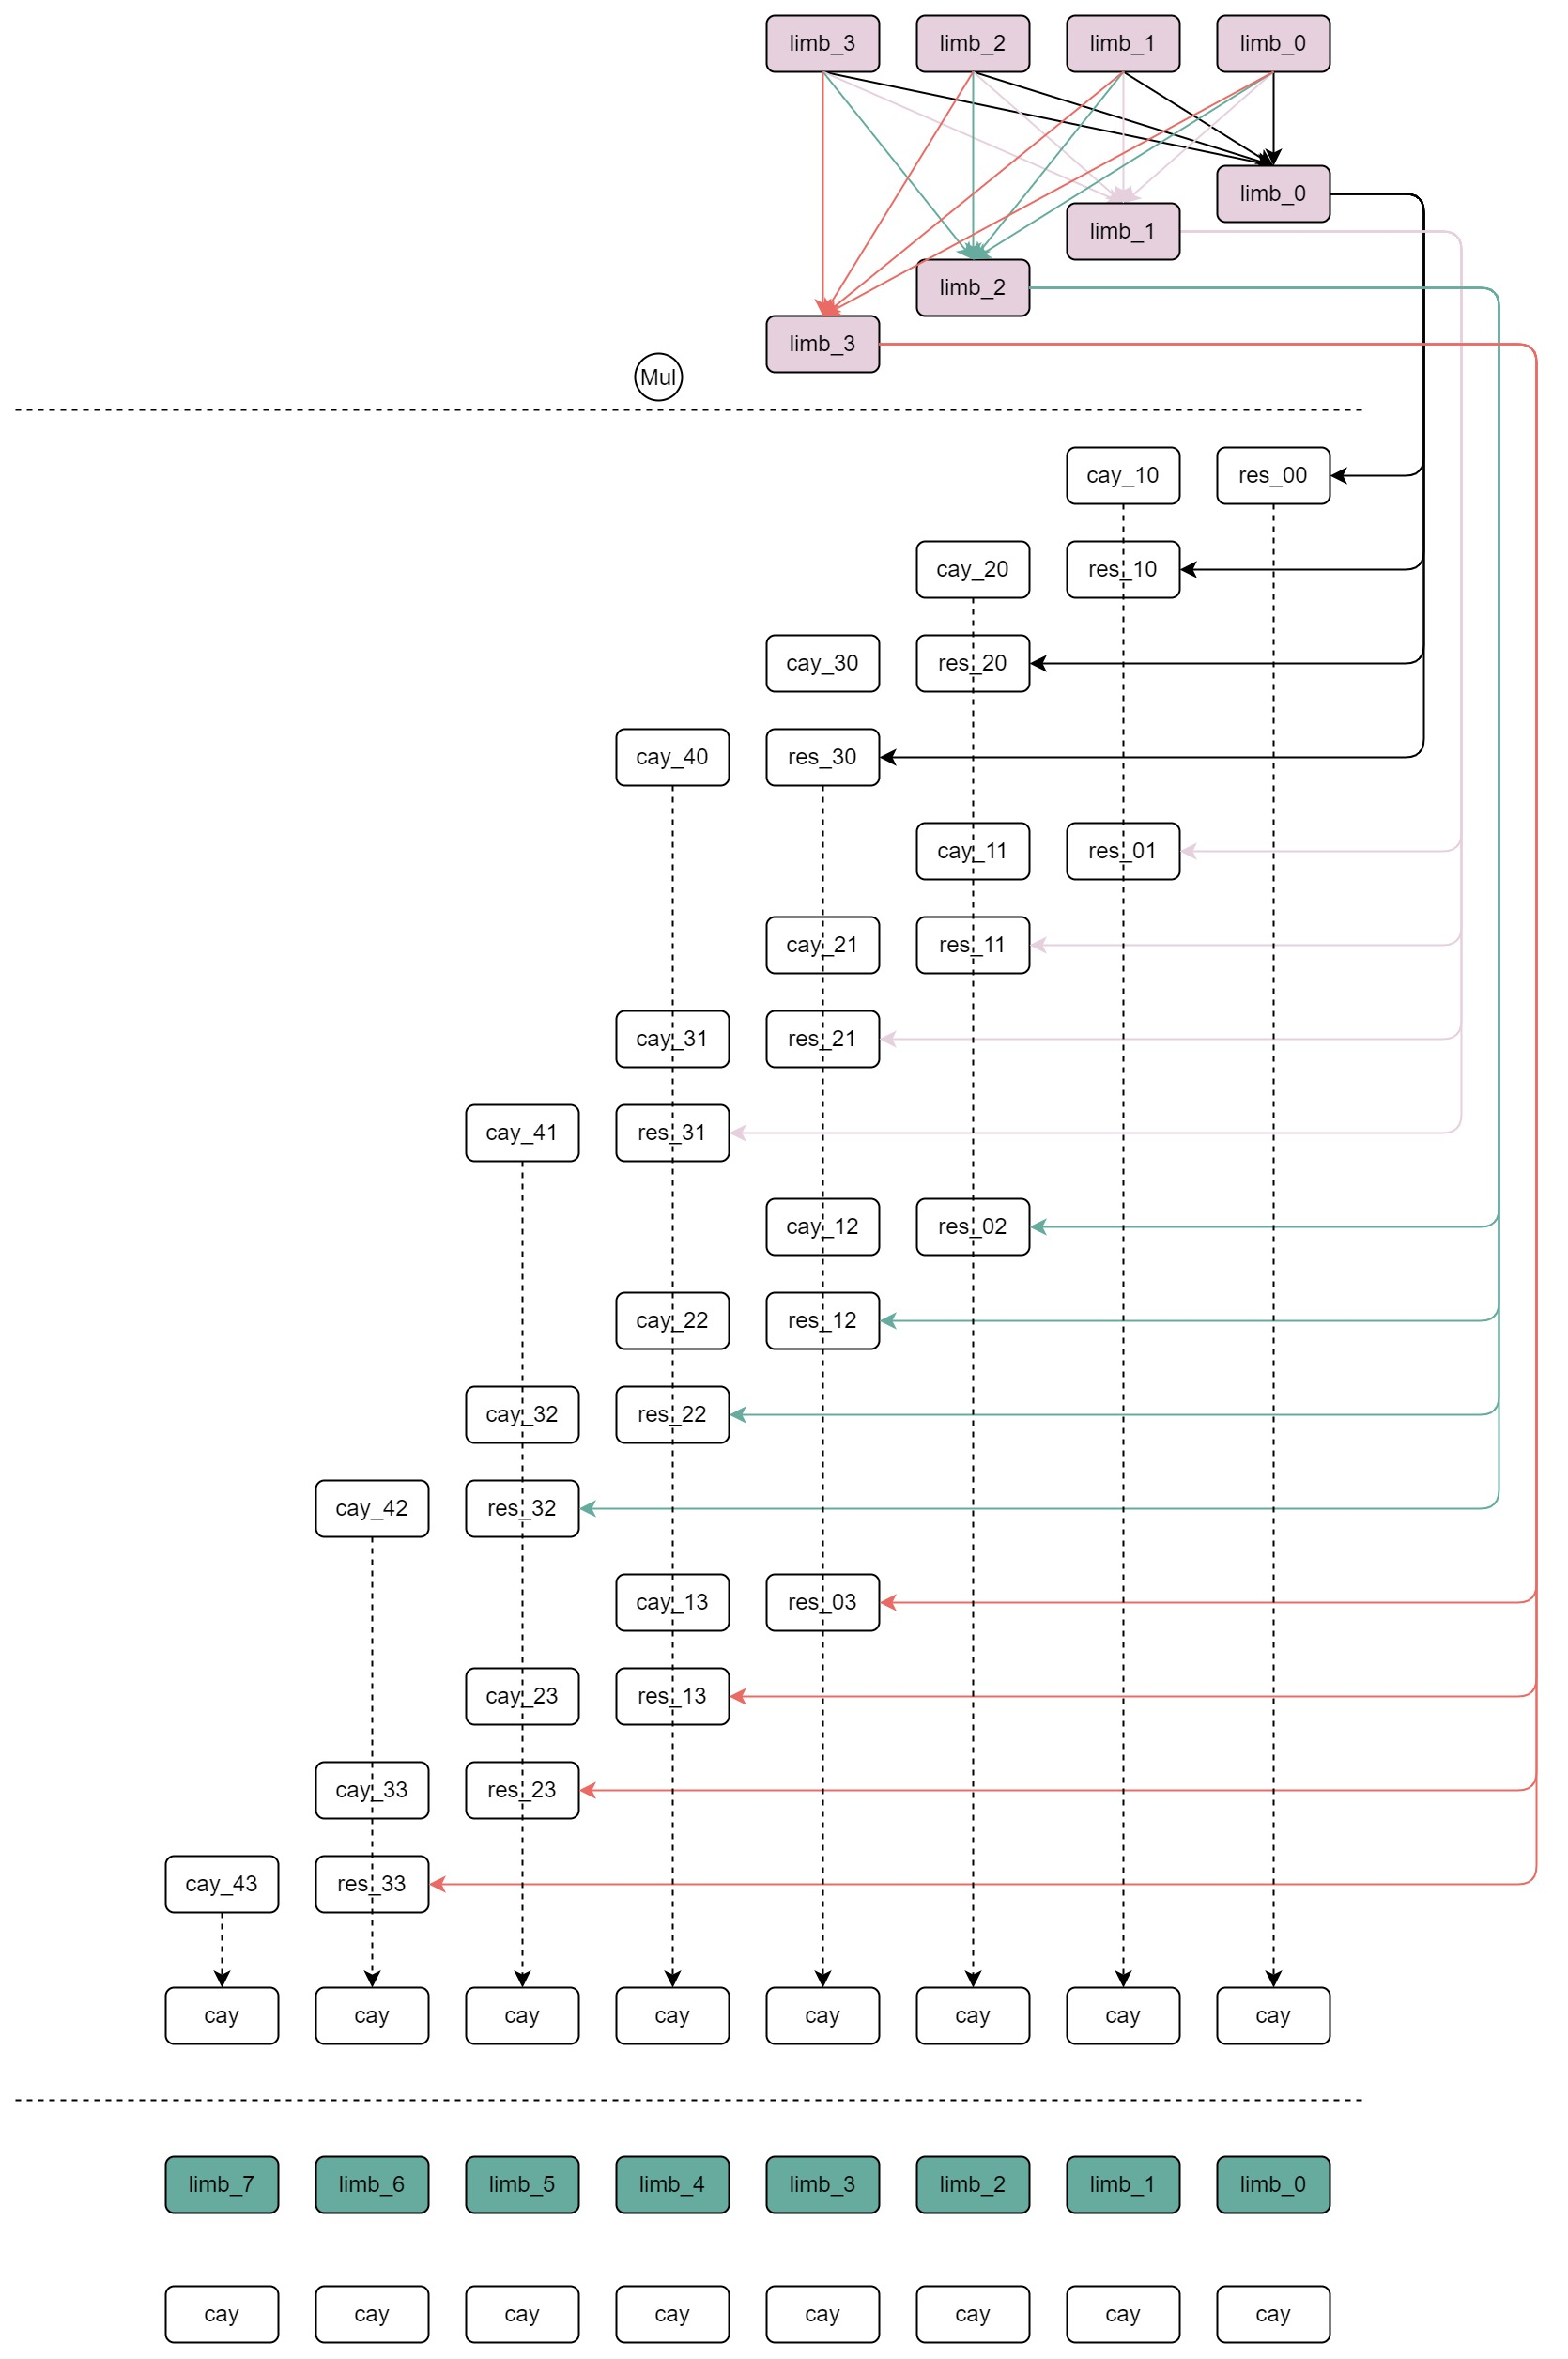
\includegraphics[width=0.8\textwidth]{mul-biguint-layout.jpg}
            \caption{Mul-biguint layout.jpg}
            \label{fig:mul-biguint-layout.jpg}
        \end{figure}
    
    \item constraints-info and costs
        \begin{itemize}
            \item Gate type num: 4
            \item Gate instance num: 9
            \item U32ArithmeticGate num: 4 * 4 + 2= 18
            \item U32AddManyGate num: 6
            \item constraints-num: 18 * (4 + 32) + (3 + 18) * (6 + 5 + 5) = 984
            \item copy-constraints: 18 * 3 + (4 + 6 + 8) * 2 + 9 = 99
            \item max-degree: 4
            \item wires-num: 18 * (6 + 32) + 6 * (3 + 18) + 5 * (5 + 18) + 5 * (7 + 18) = 1050
        \end{itemize}

\end{enumerate}